%!TEX root = report
\section{Visual Localisation}

For visual localisation, a set of 4 cameras is used. The camera's parameters such as their focal width, height and distortion factors (\textit{intrinsic parameters}) are determined using an algorithm provided by \texttt{OpenCV} (§ \ref{sec:intrinsic}). 
Using color filtering and some basic shape recognition, a set of feature or reference points are localized in the images (§ \ref{sec:imageprocessing}).
Combining these image positions with the knowledge of the exact positions in the object space, the 3D camera poses (or \textit{extrinsic parameters}) are obtained (§ \ref{sec:extrinsic}). 
Knowing the intrinsic and extrinsic parameters of the camera, any point can be located given its image. A higher robustness is achieved when the point is triangulated using its image position in more than one camera (§ \ref{sec:triangulation}).
This visual localization process is summarized in Figure \ref{fig:visual}.
\begin{figure}[H]
    \centering
    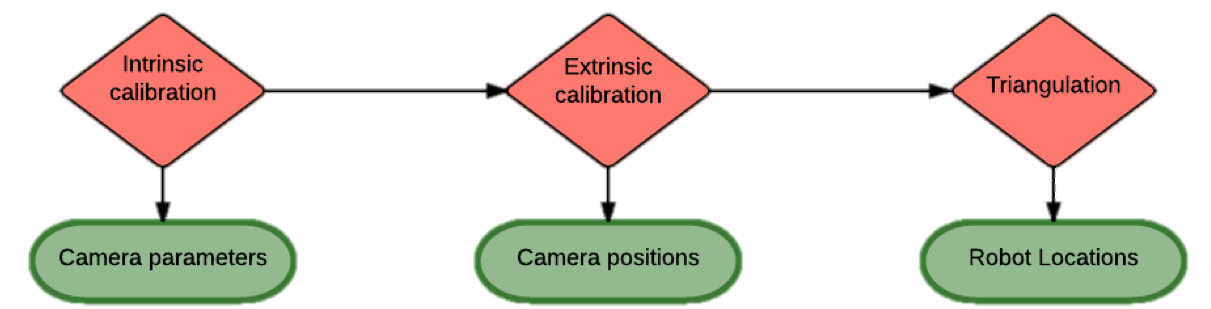
\includegraphics[width=.7\linewidth]{files/Visual.png}
    \caption{Steps of visual localization.}
    \label{fig:visual}
\end{figure}



%!TEX root = ../report.tex
\subsection{Intrinsic Calibration}

Implemented algorithm
...

%\begin{lstlisting}[caption=Listing]
%\end{lstlisting}

%\begin{figure}[H]
%	\centering
%	\begin{subfigure}[b]{0.49\linewidth}
%		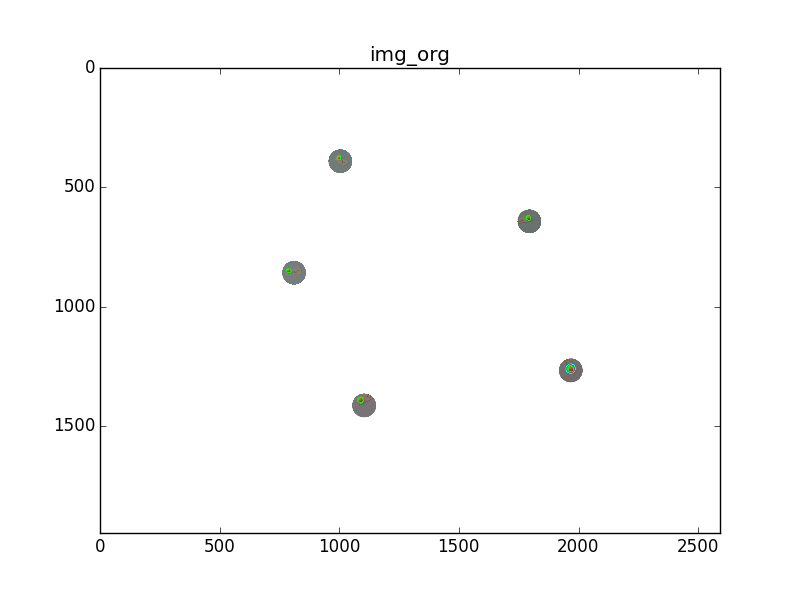
\includegraphics[width=\linewidth]{../files/img_org139.png}
%		\caption{Regions of interest chosen by user and extracted colors}
%		\label{feat_step0}
%	\end{subfigure}
%	\begin{subfigure}[b]{0.49\linewidth}
%		\includegraphics[width=\linewidth]{../files/img_h139.png}
%		\caption{\textit{Hue} representation of original image}
%		\label{feat_step1}
%	\end{subfigure}
%	\begin{subfigure}[b]{0.49\linewidth}
%		\includegraphics[width=\linewidth]{../files/img_s139.png}
%		\caption{\textit{Saturation} representation of original image}
%		\label{feat_step2}
%	\end{subfigure}
%	\begin{subfigure}[b]{0.49\linewidth}
%		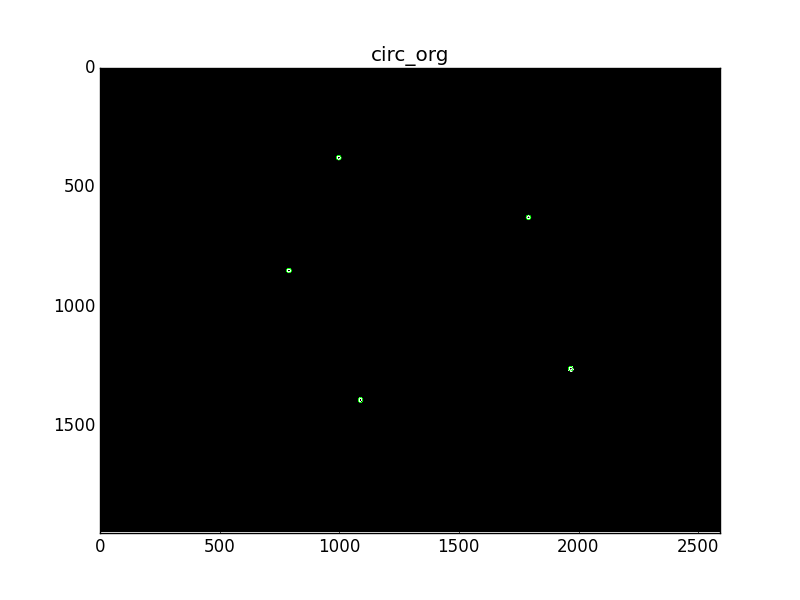
\includegraphics[width=\linewidth]{../files/circ_org139.png}
%		\caption{Regions of interest chosen by user and extracted colors}
%		\label{feat_step3}
%	\end{subfigure}
%	
%	
%	\begin{subfigure}[b]{0.49\linewidth}
%		\includegraphics[width=\linewidth]{../files/zdot_RefTrackNL.png}
%	\end{subfigure}
%	\begin{subfigure}[b]{0.49\linewidth}
%		\includegraphics[width=\linewidth]{../files/speeds_RefTrackNL.png}
%	\end{subfigure}
%	\begin{subfigure}[b]{0.49\linewidth}
%		\includegraphics[width=\linewidth]{../files/xyz_RefTrackNL.png}
%	\end{subfigure}
%	\caption{Procedure for feature extraction} 
%	\label{features}
%\end{figure}

%!TEX root = report.tex
\subsection{Image Processing}
\label{sec:imageprocessing}

The implemented procedure to detect the image of the robot head and the reference points is based on bright colored, circular reference points and is semi-automatic.

\begin{figure}[htb]
	\begin{subfigure}[b]{0.49\linewidth}
        \centering
		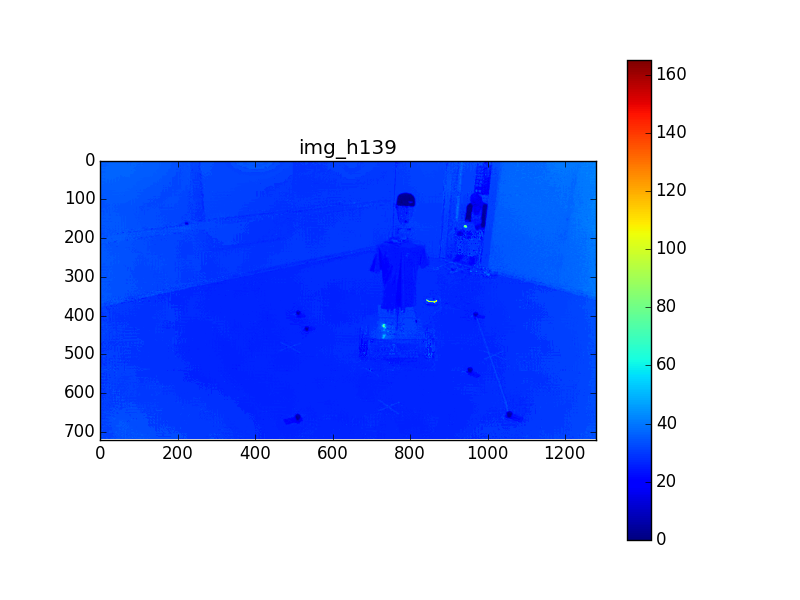
\includegraphics[width=\linewidth]{files/_img_h139.png}
		\caption{\textbf{Hue} representation of original image}
		\label{fig:img_h}
	\end{subfigure}
	\begin{subfigure}[b]{0.49\linewidth}
        \centering
		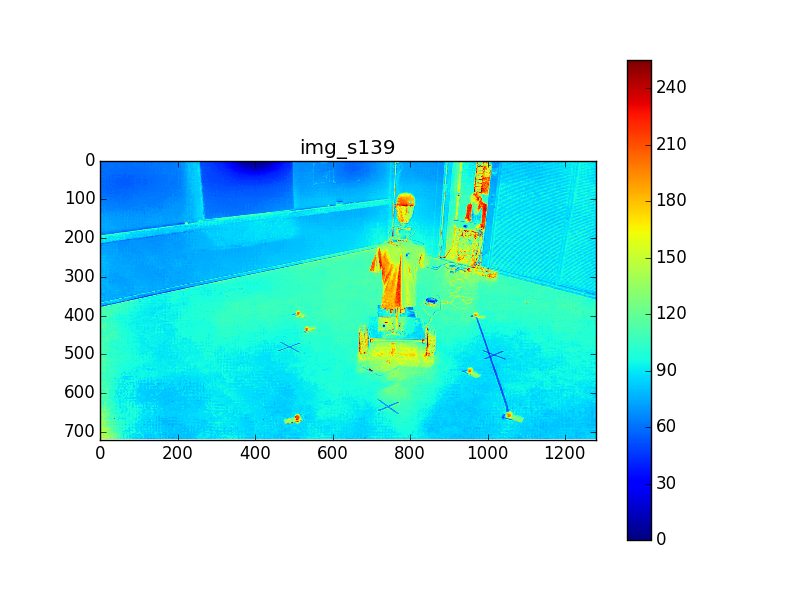
\includegraphics[width=\linewidth]{files/_img_s139.png}
		\caption{\textbf{Saturation} representation of original image}
		\label{fig:img_s}
	\end{subfigure}
    \caption{HSV components used for color extraction.}
\end{figure}
Examining the picture's HSV representation (Figures \ref{fig:img_h} and \ref{fig:img_s}), one can see that a combination of the H and S values gives a good criteria for the extraction of the bright colored points. 

The user defines the regions of interest and the relative position of the reference points by clicking on these points in the order of their numbering.
The colors in these regions of interest are extracted in two steps: first a rough filter is applied to the image which filters out any pixels that lie outside of a certain color range and sets their values to 0.
The color distribution of the left over pixels is then characterized by its mean $\mu$ and standard deviation $\sigma$ and only colors lying above and below a certain threshold are preserved. Formally the criterion for pixels that are kept is

\begin{equation}
    \frac{I(x,y)-\mu}{\sigma}\leq z.
\end{equation}

A good value for the threshold $z$ was empirically found to be 2.

The contours of the resulting binary image undergo two tests. 
First, the area within the contour has to lie above a empirically found minimum for the contour to be further treated. The resulting contours and the regions of interest are shown in Figure \ref{fig:img_org}. 

\begin{figure}[htb]
	\centering
	\begin{subfigure}[b]{0.49\linewidth}
        \centering
		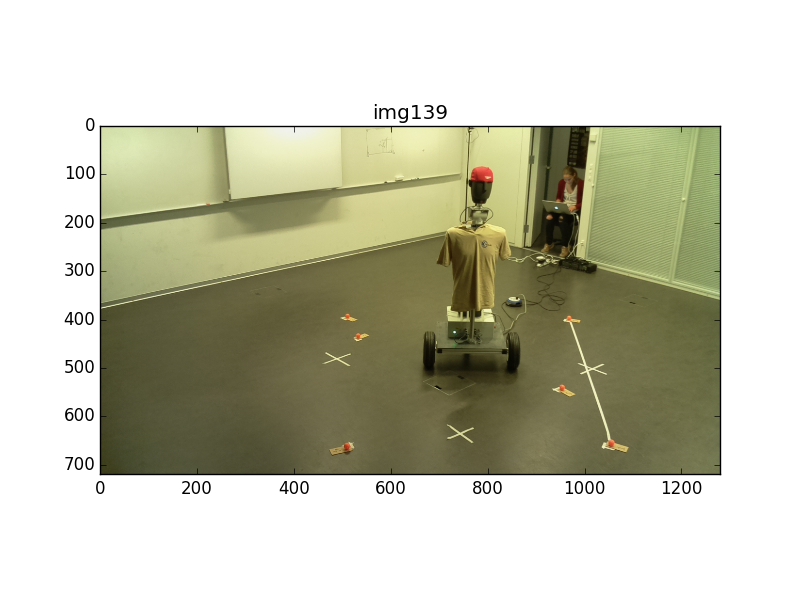
\includegraphics[width=\linewidth]{files/_img139_cvt.png}
		\caption{Original image}
		\label{fig:img}
	\end{subfigure}
	\begin{subfigure}[b]{0.49\linewidth}
        \centering
		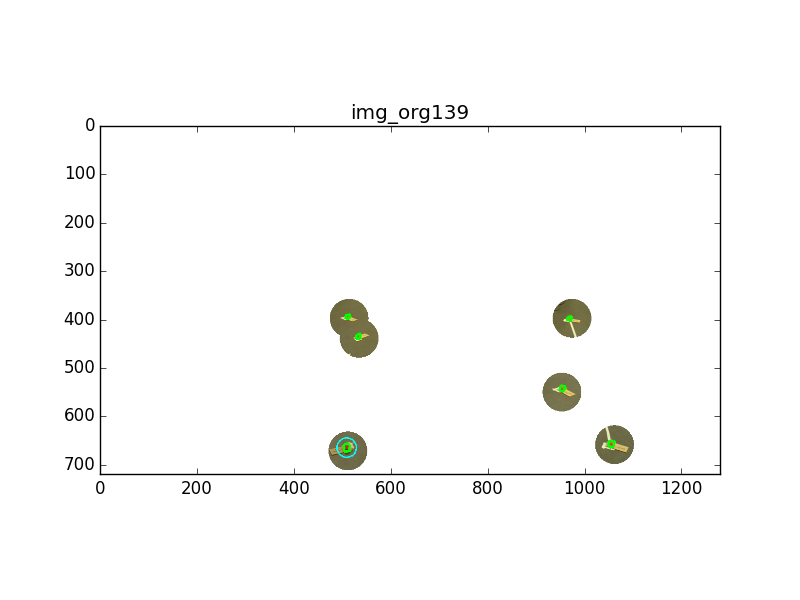
\includegraphics[width=\linewidth]{files/_img_org139.png}
		\caption{Regions of interest and extracted colors}
		\label{fig:img_org}
	\end{subfigure}
    \caption{Extraction of regions of interest for reference points.} 
\end{figure}

Secondly, the circular shape is tested by placing a circular filter of an approximate radius onto the contours and counting the white pixels that lie inside the circle and outside the circle respectively (true positives and false positives). 
The proportion of true positives has to lie above a certain threshold $t$ for the contour to be considered valid.  
The resulting binary image is composed of at least $N_{pts}$ contours whose centroids can be obtained by calculating the respective moments $M_{i,j}=\sum_{x} \sum_{y} x^iy^i I(x,y)$ ($x$, $y$ correspond to pixel coordinates and $I(x,y)$ is the pixel intensity). 
The centroid coordinates are given by $\bar{x}=M_{10}/M_{00}$ and $\bar{y}=M_{01}/M_{00}$. If two centroids are too close to each other, they are considered as duplicate and repliced by their midpoint.

The resulting binary images with the final centroids for each point of both reference points and the robot head are shown in Figures \ref{fig:circ_org} and \ref{fig:circ_red} respectively.

\begin{figure}[htb]
	\begin{subfigure}[b]{0.49\linewidth}
        \centering
		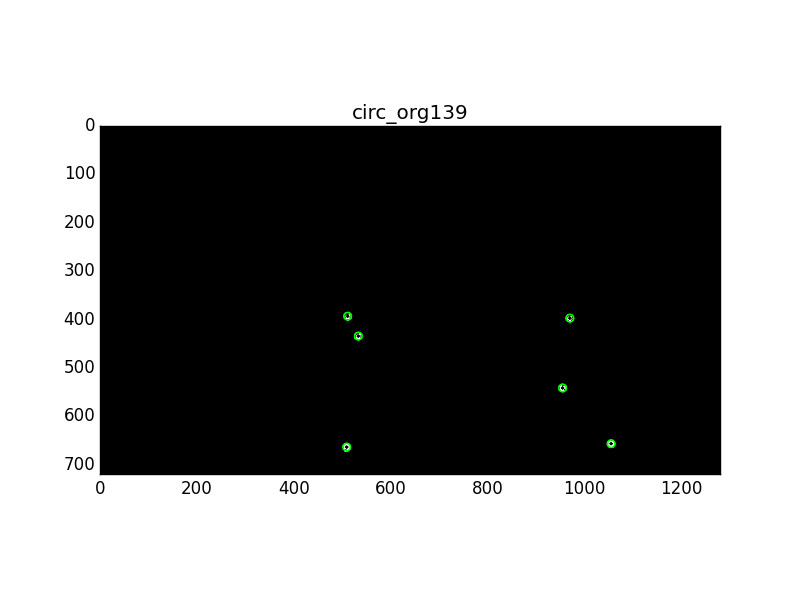
\includegraphics[width=\linewidth]{files/_circ_org139.png}
		\caption{Extracted colours, reference points}
		\label{fig:circ_org}
	\end{subfigure}
	\begin{subfigure}[b]{0.49\linewidth}
        \centering
		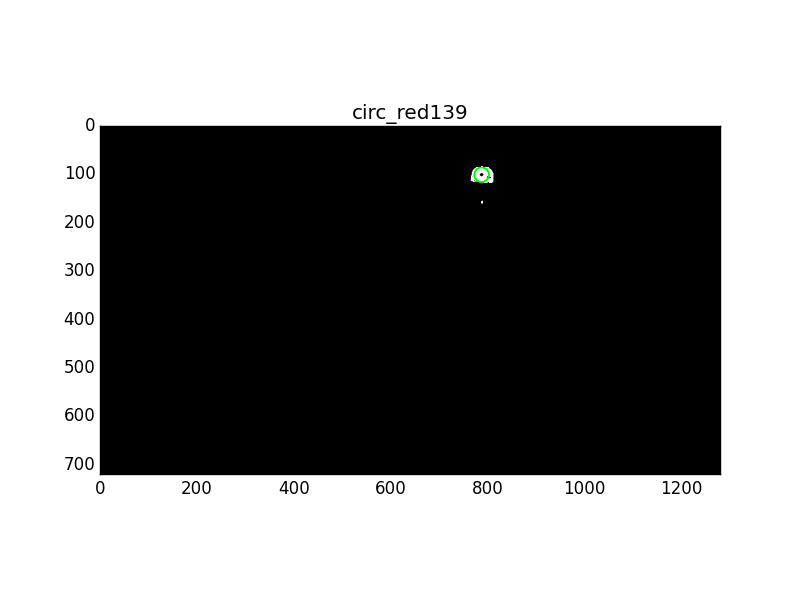
\includegraphics[width=\linewidth]{files/_circ_red139.png}
		\caption{Extracted colours, robot head}
		\label{fig:circ_red}
	\end{subfigure}
	\caption{Final results of image processing for feature extraction.} 
\end{figure}

%\begin{lstlisting}[caption=Listing]
%\end{lstlisting}


%!TEX root = report.tex
\subsection{Extrinsic Calibration}
\label{sec:extrinsic}
\subsubsection{Reference points}

\paragraph{Points} 
In a first run, 4 to 6 bright orange circular reference points where used for the extrinsic calibration. The points are numbered and the first 2 points serve as the basis for the reference frame. (see Figure \ref{fig:ref_points}).

Since the distances between all points can be very accurately measured using a laser pointer, the euclidean distance matrix is set up and the absolute positions in the reference frame are obtained using the classical Multidimensional Scaling (MDS) method. \cite{Wickelmaier2003}

The limitations of this method are that the number of reference points can only hardly be extended since all points need to be numbered manually by the user and the number of laser pointer measurements increases quadratically.
Secondly, the radius of the reference points needs to be chosen big enough to be robustly detected from distance. But increasing the radius, leads to a higher imprecision since the points can not be exactly placed on the ground and are perceived at different heights from different camera angles.

\paragraph{Checkerboard}
A second and more user friendly approach using a checkerboard for reference points was implemented in a second run. 
Since many robust implementations exist for checkerboard corner detection, its use promises a big number of reference points with minimal effort and high reliability. 
In addition to that, the checkerboard corners are of much smaller radius than circular reference points and can be placed exactly on the ground.

In order to avoid the manual numbering of all checkerboard points an automatic procedure based on three reference points placed in the corners of the checkerboard is implemented. 
The three reference points are detected manually and the numbering starts at the chessboard corner closest to point 1, goes on in direction of point 2 and then up in direction of point 3 (Figure \ref{fig:ref_checkerboard.png}).

\begin{figure}[htb]
	\centering
	\begin{subfigure}[b]{0.49\linewidth}
        \centering
		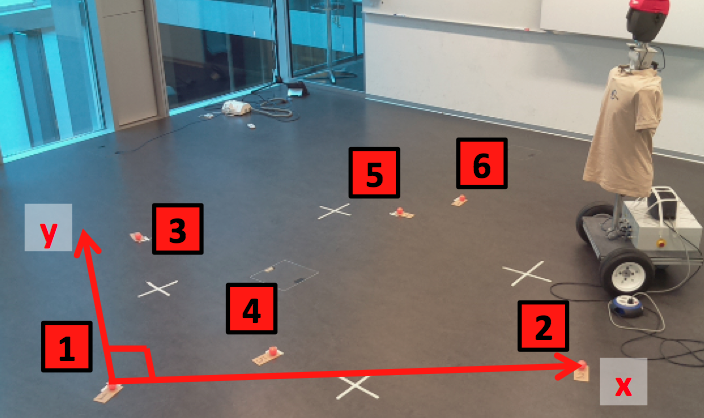
\includegraphics[height=0.6\linewidth]{files/ref_points.png}
		\caption{Reference points reference frame}
        \label{fig:ref_points}
	\end{subfigure}
	\begin{subfigure}[b]{0.49\linewidth}
        \centering
		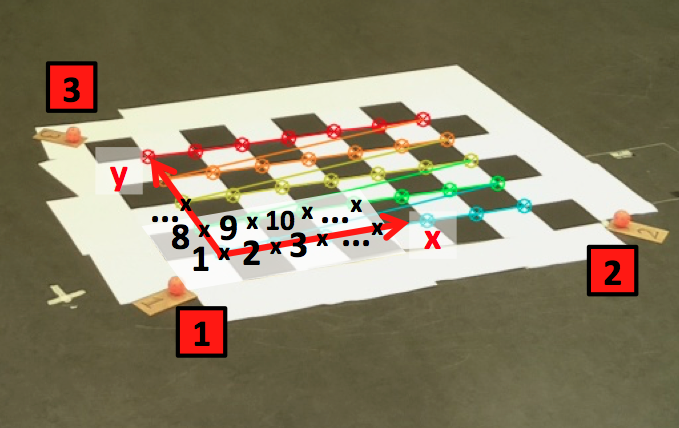
\includegraphics[height=0.6\linewidth]{files/ref_checkerboard.png}
		\caption{Checkerboard reference frame and numbering}
		\label{fig:ref_checkerboard.png}
	\end{subfigure}
	\caption{Reference point and checkerboard layout conventions.} 
\end{figure}

\paragraph{Algorithm}

The reference points are detected as explained in § \ref{sec:imageprocessing}. The so found image-object space correspondances can be used to determine the camera position and orientation by solving the following system of equations for $R$ and $\mathbf{t}$.
\begin{align}
    \mathbf{x_i} = proj(\mathbf{X_i},P)& = C \quad P \quad \mathbf{X_i} \\
    s_i \begin{bmatrix} u_i \\ v_i \\ 1 \end{bmatrix} &= 
    C \begin{bmatrix} R \quad|\quad \mathbf{t} \end{bmatrix}
    \begin{bmatrix} X_i \\ Y_i \\  Z_i \\ 1 \end{bmatrix}, \quad \text{for }i=1\cdots N_{pts},
    \label{eq:projection}
\end{align}

where $N_{pts}$ is the number of points (4 to 6 or number of checkerboard corners), 
$\begin{bmatrix} u_i & v_i & 1 \end{bmatrix} ^T$ are the homogenous image coordinates with scaling factor $s_i$ and $\begin{bmatrix} X_i & Y_i &  Z_i & 1 \end{bmatrix} ^T$ are the homogenous object point cooridnates. $C$ is the intrinsic camera matrix, determined as explained in \ref{sec:intrinsic}.

The extrinsic camera matrix $P$ that one needs to solve for can be decomposed in a rotation and a translation component.
\begin{align}
    R &= \begin{bmatrix} 
        r_{11} & r_{12} & r_{13} \\
        r_{21} & r_{22} & r_{23} \\
        r_{31} & r_{32} & r_{33} \\
    \end{bmatrix} \quad \text{Camera rotation matrix}\\
    \mathbf{t} &= \begin{bmatrix} 
        t_1 & t_2 & t_3
    \end{bmatrix} ^T \quad \text{Camera translation vector}
    \label{eq:solvepnp}
\end{align}

The camera center in object space coordinates is then given by

\begin{equation}
    \begin{bmatrix} x_C & y_C & z_C \end{bmatrix}^T = -R^{-1} \mathbf{t}.
\end{equation}

There are 12 unknowns and each new point provides 3 independant equations. Therefore at least 4 points are requried for solving this problem.

Various methods have been proposed for solving this Perspective-$n$-Point or P$n$P problems. 
The methods can be embedded in a Ransac scheme, which makes them more resistant to outliers. 
However, outliers will not occur in the present experimental setup because of its deterministic nature: all reference points are precisely defined and need to be detected, as opposed to setups where a undefined amount of feature points are extracted from images.

Three different methods for solving this P$n$P problem are implemented in OpenCV.
\texttt{P3P} is based on a technique that is limited to 4 points only, so it was immediately rejected. The \texttt{EPNP} method \cite{Lepetit2009} provides a non-iterative solution to the problem which is more stable and computationally inexpensive. Since in the present case, the number of points is limited to 40 and the calculation time turned out to be acceptable, the method chosen is the \texttt{ITERATIVE} method, based on reprojection error minimization.

The reprojection error is the sum of the squared distances between observed projections $\mathbf{x_i}=[u_i,v_i,1]^T$ and the projected object points ($\mathbf{proj}(\mathbf{X_i},P)$), defined as in \eqref{eq:projection} and calculated with the current estimation of the extrinsic camera matrix $P$. Formally, this means

\begin{equation}
S(\boldsymbol\beta) = \sum_{i=1}^{N_{pts}} \| \mathbf{x_i}-proj(\mathbf{X_i},P(\boldsymbol\beta)) \| ^2 ,
\end{equation}

and the optimization problem can be written as
\begin{equation}
    \hat{\boldsymbol\beta} = \underset{\beta} {\mathrm{argmin}} ~S(\boldsymbol\beta).
\end{equation}

For an adequate convergence in all directions, this minimization problem is solved with the Levenberg-Marquardt algorithm, also called damped least-squares. The optimization parameters are the entries of the matrix $P$, which are grouped in the vector $\boldsymbol\beta$. At each minimization step a \"damped\" update of the parameter vector $\boldsymbol\beta=\boldsymbol\beta_{old}+\boldsymbol\delta=$ is used depending on the decent of the optimization function, as defined in \eqref{eq:LMA} \cite{LMA}
\begin{equation}
    (J^TJ + \lambda \mathbf{diag}(J^TJ))\boldsymbol\delta = J^T[\mathbf{x}-\mathbf{proj}(\mathbf{X},P)]
\label{eq:LMA}
\end{equation}

where $J$ is the Jacobian matrix of the reprojection function and $\lambda$ is the damping factor. It is tuned such that
the convergence is moderated in the case of very fast descending functions, preventing from instability, and enhanced for slowly converging problems.

%!TEX root = report.tex
\subsection{Triangulation}
\label{sec:triangulation}

The basics for the triangulation technique are the camera projection equations \eqref{eq:projection}.
The difference is that in this case, one wants to find the real position of one point given its image points in images from multiple cameras. The governing equation is thus given by

\begin{align}
    \mathbf{x_j} & = C \quad P \quad \mathbf{X} \\
    s_j \begin{bmatrix} u_j \\ v_j \\ 1 \end{bmatrix} &= 
    C \begin{bmatrix} R \quad|\quad \mathbf{t} \end{bmatrix}
    \begin{bmatrix} X \\ Y \\  Z \\ 1 \end{bmatrix}, \quad \text{for }j=1\cdots N_{cameras}.
    \label{eq:triangulation}
 \end{align}

Both cases with fixed or free height $Z$ are considered. The resulting system of equations has 2 or 3 unknowns. 
The method applied is the one proposed by Hartley Zisserman (\cite{hz}, Chapter 12.2). 
First of all, for each camera, the following matrix needs to be set up. 

\begin{equation}
    \mathbf{A_j} = \begin{bmatrix} u_j \mathbf{f_3}-\mathbf{f_1} \\ v_j \mathbf{f_3}-\mathbf{f_2} \end{bmatrix},
\end{equation}

where $\mathbf{f_k}=P(k,:)$ denotes the $k$th row of the projection matrix and $u_j$,$v_j$ are the image points of the required point in Camera $j$.
The matrix $A$ is then composed of all rows $\mathbf{A_j}$, vertically stacked. It is of size $4\times(2 N_{cameras}$).

If the height is specified, then finding the solution to \eqref{eq:triangulation} comes back to solving

\begin{align}
    A'\mathbf{x}&=\mathbf{b}\\  
    \begin{bmatrix} \mathbf{a_1} & \mathbf{a_2} \end{bmatrix}^T \mathbf{x} &= -\mathbf{a_3}Z-\mathbf{a_4},
\end{align}

where $f_k$ denotes the $k$th row of the matrix $\mathbf{A}$
This system of equations can be solved in the least-squares sense, which leads to the solution $\mathbf{\hat{x}}=(A^TA)^{-1}A^T\mathbf{b}^T$. 
Adding the third component Z to $\mathbf{\hat{x}}$, the solution is obtained.

If the height is not specified, one can simply use a single value decomposition of $A$. The eigenvector with biggest eigenvalue corresponds to the solution of \eqref{eq:triangulation} in the least squares sense.

%\begin{lstlisting}[caption=Listing]
%\end{lstlisting}

%\begin{figure}[htb]
%	\centering
%	\begin{subfigure}[b]{0.49\linewidth}
%		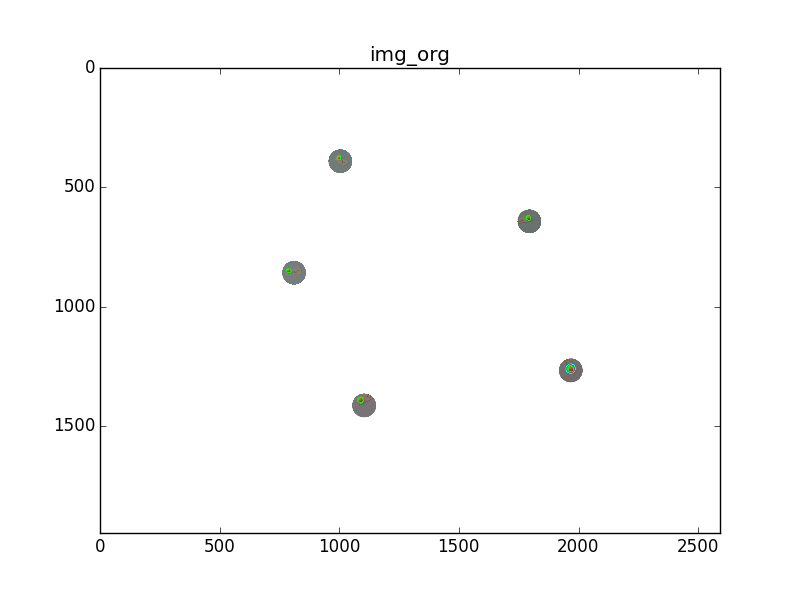
\includegraphics[width=\linewidth]{../files/img_org139.png}
%		\caption{Regions of interest chosen by user and extracted colors}
%		\label{feat_step0}
%	\end{subfigure}
%	\begin{subfigure}[b]{0.49\linewidth}
%		\includegraphics[width=\linewidth]{../files/img_h139.png}
%		\caption{\textit{Hue} representation of original image}
%		\label{feat_step1}
%	\end{subfigure}
%	\begin{subfigure}[b]{0.49\linewidth}
%		\includegraphics[width=\linewidth]{../files/img_s139.png}
%		\caption{\textit{Saturation} representation of original image}
%		\label{feat_step2}
%	\end{subfigure}
%	\begin{subfigure}[b]{0.49\linewidth}
%		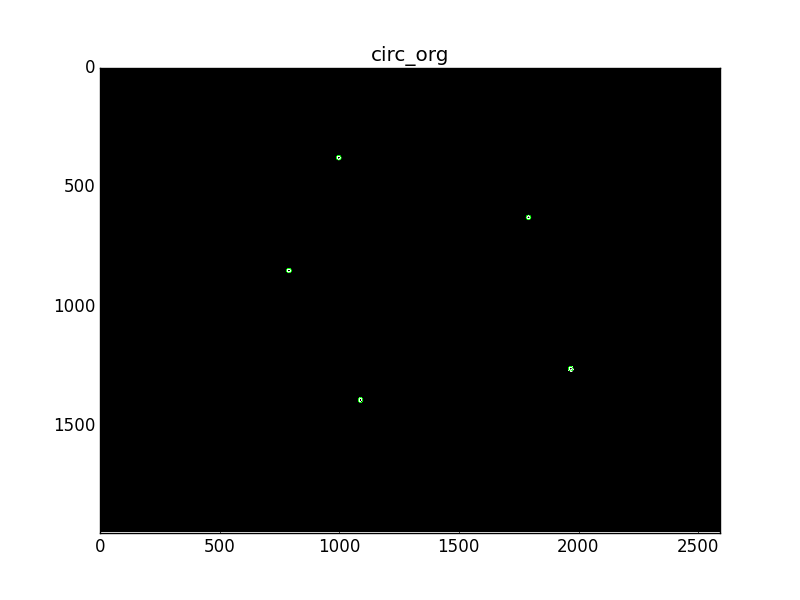
\includegraphics[width=\linewidth]{../files/circ_org139.png}
%		\caption{Regions of interest chosen by user and extracted colors}
%		\label{feat_step3}
%	\end{subfigure}
%	
%	
%	\begin{subfigure}[b]{0.49\linewidth}
%		\includegraphics[width=\linewidth]{../files/zdot_RefTrackNL.png}
%	\end{subfigure}
%	\begin{subfigure}[b]{0.49\linewidth}
%		\includegraphics[width=\linewidth]{../files/speeds_RefTrackNL.png}
%	\end{subfigure}
%	\begin{subfigure}[b]{0.49\linewidth}
%		\includegraphics[width=\linewidth]{../files/xyz_RefTrackNL.png}
%	\end{subfigure}
%	\caption{Procedure for feature extraction} 
%	\label{features}
%\end{figure}

\newpage
%!TEX root = report.tex

\subsection{Performance Measure}
The performance of the localization can be quantified by the distance from the calculated target point to its real position (measured with a laser pointer). 
Both algorithms, fixed-height and free-height (see § \ref{sec:triangulation}), are applied. The errors in the x-y plane for fixed-height and free-height as well as the 3D error for free-height are considered. 

With the four available cameras there are several camera combinations that can be used for the calculation.
It was found that the error in the position of the robot is highly dependent on which cameras are used for triangulating the image points. 
Currently, the best camera combination is determined based on the error between the measured and actual position of the robot.
In later experimental setups, however, the real position of the robot will not be directly measured, so it is necessary to find another criterion for evaluating the camera combinations.
One option considered was to use the errors of the reprojection of the reference points, whose positions are already well-known.
The results of this approach, shown in Figure~\ref{fig:res0_err}, however, suggest that the correlation between the reference point error and the robot position error is not strong enough, so a different criterion needs to be found.
This task is beyond the scope of the present project so in the following section, all camera combinations are considered and the real position of the robot is used for measurement of performance.


\begin{figure}[H]
    \centering
    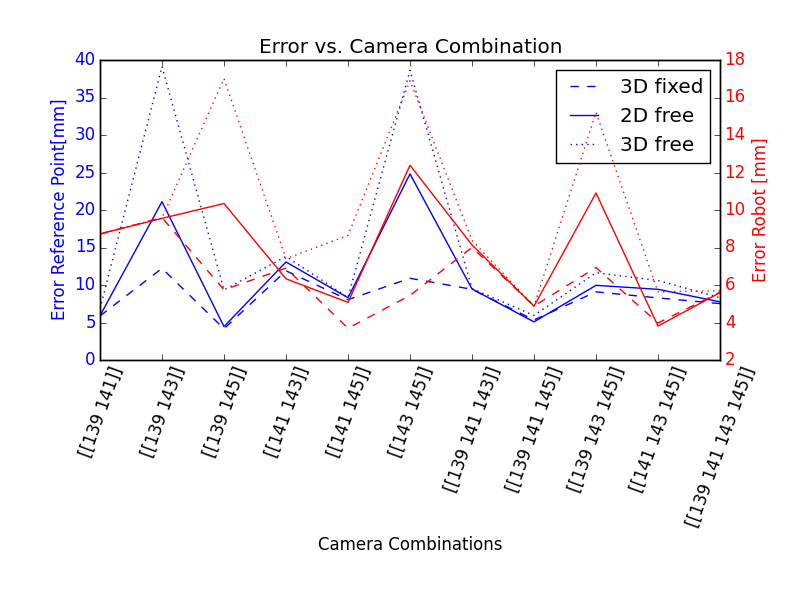
\includegraphics[width=.8\linewidth]{files/res0_combi_4.png}
    \caption{Experiment in Atrium: results of visual localization for various camera combinations.}
    \label{fig:res0_err}
\end{figure}

%\begin{lstlisting}[caption=Listing]
%\end{lstlisting}

%\begin{figure}[htb]
%	\centering
%	\begin{subfigure}[b]{0.49\linewidth}
%		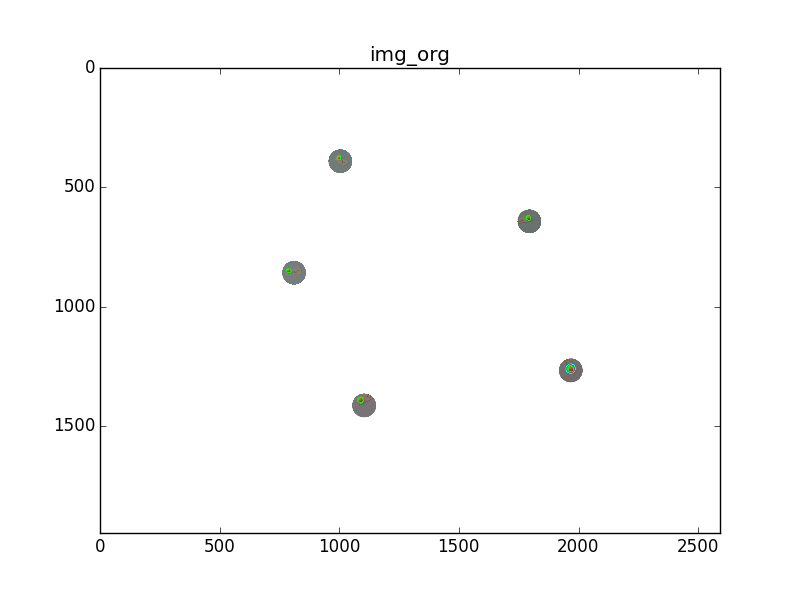
\includegraphics[width=\linewidth]{../files/img_org139.png}
%		\caption{Regions of interest chosen by user and extracted colors}
%		\label{feat_step0}
%	\end{subfigure}
%	\begin{subfigure}[b]{0.49\linewidth}
%		\includegraphics[width=\linewidth]{../files/img_h139.png}
%		\caption{tit{Hue} representation of original image}
%		\label{feat_step1}
%	\end{subfigure}
%	\begin{subfigure}[b]{0.49\linewidth}
%		\includegraphics[width=\linewidth]{../files/img_s139.png}
%		\caption{tit{Saturation} representation of original image}
%		\label{feat_step2}
%	\end{subfigure}
%	\begin{subfigure}[b]{0.49\linewidth}
%		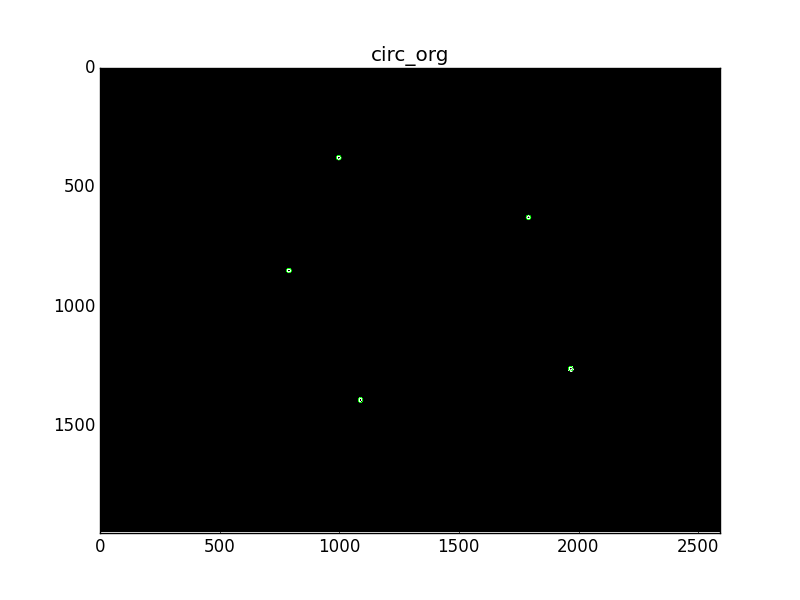
\includegraphics[width=\linewidth]{../files/circ_org139.png}
%		\caption{Regions of interest chosen by user and extracted colors}
%		\label{feat_step3}
%	\end{subfigure}
%	
%	
%	\begin{subfigure}[b]{0.49\linewidth}
%		\includegraphics[width=\linewidth]{../files/zdot_RefTrackNL.png}
%	\end{subfigure}
%	\begin{subfigure}[b]{0.49\linewidth}
%		\includegraphics[width=\linewidth]{../files/speeds_RefTrackNL.png}
%	\end{subfigure}
%	\begin{subfigure}[b]{0.49\linewidth}
%		\includegraphics[width=\linewidth]{../files/xyz_RefTrackNL.png}
%	\end{subfigure}
%	\caption{Procedure for feature extraction} 
%	\label{features}
%\end{figure}
